\section{Widening the latent space delays memorization}
\label{sec:phenomenon}

\Cref{fig:phenomenon-main}(a) shows the final memorized fraction after 5M steps as the latent dimension is swept from $\dlat=5$, equal to the intrinsic dimension, to $\dlat=40$ at a fixed hidden width of $256$, five seeds per width (setup in \cref{sec:setup}). Once $\dlat$ exceeds $\dint$ the fraction falls monotonically: $30.0$, $21.7$, $17.1$, $12.7$, $8.0$, $3.7$, $1.6$, $0.8$, $0.3$ and $0.1\%$ at $\dlat=5,8,10,12,15,20,25,30,35,40$. The added coordinates carry only isotropic noise, so the signal the network has to learn is the same at every width; what changes is how quickly it fits its training set. Holding the width fixed matters: scaling the hidden width with $\dlat$ turns the sweep into a capacity sweep and no longer isolates the latent dimension.

\begin{figure}[t]
  \centering
  \begin{subfigure}{0.46\linewidth}
    \centering
    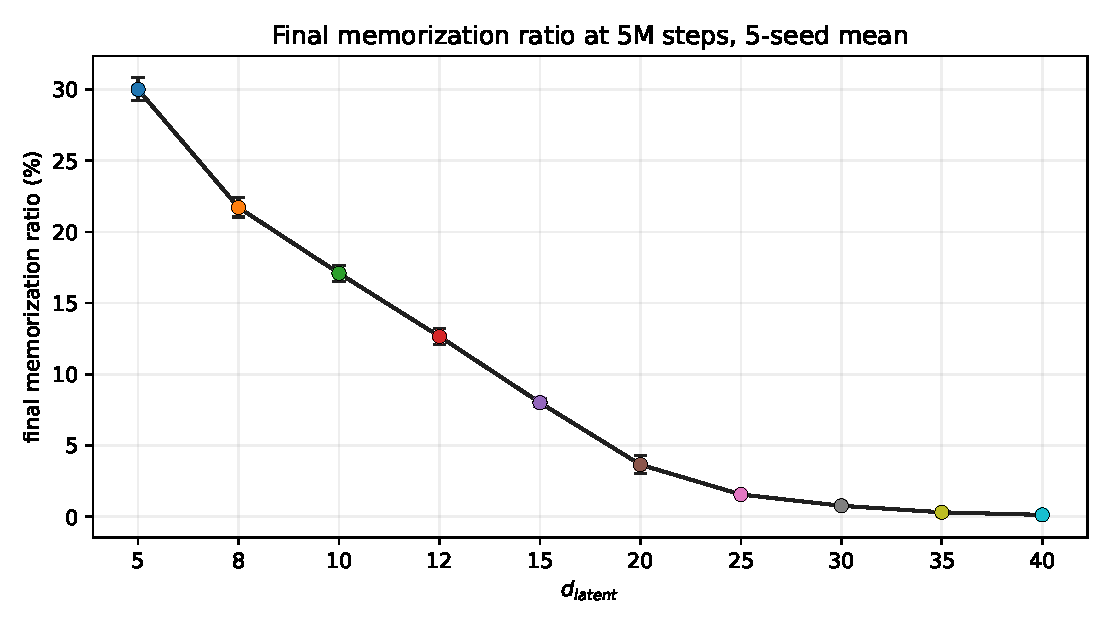
\includegraphics[width=\linewidth]{figures/synthetic_mlp_final_mem_ratio.pdf}
    \caption{Final memorized fraction.}
  \end{subfigure}\hfill
  \begin{subfigure}{0.52\linewidth}
    \centering
    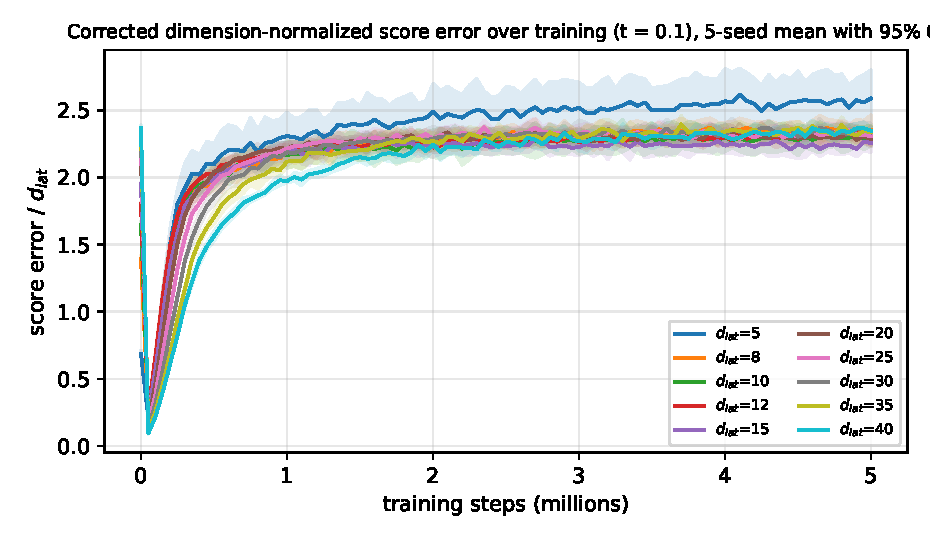
\includegraphics[width=\linewidth]{figures/synthetic_mlp_score_error_per_dim.pdf}
    \caption{Population score error per coordinate.}
  \end{subfigure}
  \caption{\textbf{Widening the latent space delays memorization.} Fixed-width MLP, $\dint=5$, five seeds, 5M steps. (a) Final memorized fraction falls from $30\%$ at $\dlat=5$ to $0.1\%$ at $\dlat=40$. (b) Population score error at $t=0.1$ per coordinate against the exact GMM score on held-out data. Every width reaches its minimum by 50k steps and then rises as the network fits its training set; the rise starts later at larger $\dlat$, and by 5M steps all widths have reached a similar level. The panel shows a delay, not a preserved score.}
  \label{fig:phenomenon-main}\label{fig:synthetic-mlp-main}
\end{figure}

The same delay is visible in score space, where the synthetic setting provides an exact target. \Cref{fig:phenomenon-main}(b) reports the population score error at $t=0.1$ per coordinate, against the exact GMM score on held-out data. Every width reaches its minimum by the first evaluation at 50k steps and then rises as the network fits its training set. The rise starts later at larger $\dlat$: the error crosses $2.0$ per coordinate at $0.35$M steps for $\dlat=5$ and at $1.05$M for $\dlat=40$, the same ordering as the memorization onset in panel (a). By 5M steps every width up to $40$ has converged to about $2.3$ per coordinate, so the final value is flat in $\dlat$ while the timing differs. Extending the same fixed-width sweep to $\dlat=240$ (\cref{fig:app-synthetic-mlp-score}) makes the delay monotone over the full range. Measured as the time for the error to double from its minimum, it is at most 100k steps for $\dlat\le40$, $200$k at $\dlat=60$, $500$k at $80$, $800$k at $100$, $1.55$M at $120$, $2.5$M at $140$, and is not reached within 5M steps for $\dlat\ge160$; beyond $\dlat\approx60$ the per-coordinate error has not returned to its small-$\dlat$ plateau by the horizon, ending at $2.59$ for $\dlat=5$ but $0.53$ for $\dlat=240$. The delay exceeds $25\times$ across the sweep.

\paragraph{The decline is not a metric artifact.}
A nearest-neighbour ratio test can lose sensitivity as the dimension grows, so the decline in panel (a) could in principle reflect the test rather than the model. \Cref{tab:projection-main} rules this out. A sampler that reproduced a training point's signal coordinates while redrawing its null coordinates would be invisible to the full-space test for $\dlat\ge10$: such signal copies are detected at $57\%$ at $\dlat=5$ but at $0.8\%$ and $0.0\%$ beyond. Repeating the test after projecting generated and training points onto the true $\dint$-dimensional signal subspace, where signal copies are detected at every width, gives $29.5\%$, $16.9\%$, $5.8\%$ and $1.2\%$ for the model samples at $\dlat=5,10,20,40$, against a $0.5\%$ chance level from fresh population draws. The models do not make signal-only copies: the decline is $25\times$ in the signal subspace, and the full-space test overstates it only mildly ($3.8$ against $5.8\%$ at $\dlat=20$, $0.1$ against $1.2\%$ at $40$). The full table, including the exact-copy control, is \cref{tab:e2-projection}.

\begin{table}[t]
  \centering\small
  \caption{Dimension-controlled memorization test (5M steps, two seeds, 5000 samples each). The ratio test of \cref{app:protocol} is applied in the full latent space and after projecting generated and training points onto the $\dint=5$ signal coordinates. Signal copies reproduce a training point's signal coordinates and redraw its null coordinates. $\alpha$ is the alignment of the learned score with the empirical score of the training set (signal coordinates, $t=0.1$). Full version: \cref{tab:e2-projection}.}
  \label{tab:projection-main}
  \begin{tabular}{lcccc}
    \toprule
     & $\dlat=5$ & $10$ & $20$ & $40$\\
    \midrule
    model samples, full-space test & $29.5\%$ & $16.7\%$ & $3.8\%$ & $0.1\%$\\
    model samples, signal-projected test & $29.5\%$ & $16.9\%$ & $5.8\%$ & $1.2\%$\\
    fresh draws, signal-projected test & $0.5\%$ & $0.5\%$ & $0.5\%$ & $0.5\%$\\
    signal copies, full-space test & $57\%$ & $0.8\%$ & $0.0\%$ & $0.0\%$\\
    signal copies, signal-projected test & $57\%$ & $57\%$ & $58\%$ & $58\%$\\
    \midrule
    $\alpha$ at 5M steps & $0.76$ & $0.54$ & $0.39$ & $0.30$\\
    \bottomrule
  \end{tabular}
\end{table}

\paragraph{Alignment with the empirical score.}
The second readout needs no threshold. Let $s^\star$ be the population score, $s_{\rm emp}$ the exact score of the empirical distribution of the $n$ training points, and $s_\theta$ the learned score, all in the signal coordinates at $t=0.1$. The alignment coefficient
\begin{equation}
  \alpha=\frac{\langle s_\theta-s^\star,\,s_{\rm emp}-s^\star\rangle}{\|s_{\rm emp}-s^\star\|^2}
\end{equation}
is $0$ for the population score and $1$ for an exact fit of the training set. It reaches $0.76$, $0.54$, $0.39$ and $0.30$ at 5M steps for $\dlat=5,10,20,40$, and it passes $0.3$ more than $30\times$ later at $\dlat=40$ than at $\dlat=5$. It also explains why the final score error in \cref{fig:phenomenon-main}(b) is flat in $\dlat$ while memorization differs $25\times$: the per-coordinate gap $\|s_{\rm emp}-s^\star\|^2$ grows $3.6\times$ from $\dlat=5$ to $40$, so a smaller $\alpha$ costs as much population error.

Two independent readouts, one of them threshold-free, agree that widening the latent space delays memorization; \cref{sec:theory} asks what a solvable model says about why, and \cref{sec:real} tests the phenomenon on real data.
